% Created 2016-08-17 Wed 14:38
\documentclass[tikz]{standalone}

\usepackage[utf8]{inputenc}
\usepackage[T1]{fontenc}

\usepackage{circledsteps}

\RequirePackage{xcolor}

%% HPI color definitions according to the design manual
% These do not exactly match the RGB values used in the Powerpoint slide master due to unknown reasons
\definecolor{hpiyellow}{RGB}{246,168,0}
\definecolor{hpiorange}{RGB}{221,97,8}
\definecolor{hpired}{RGB}{177,6,58}
\definecolor{hpigray}{RGB}{90,96,101}
\definecolor{hpiblue}{RGB}{0,122,158}


\renewcommand{\sfdefault}{neosans}
% Different font weights for neosans
\newcommand{\textl}[1]{{\fontseries{l}\selectfont #1}} % light
\newcommand{\textm}[1]{{\fontseries{m}\selectfont #1}} % medium, same as default weight
\newcommand{\textsb}[1]{{\fontseries{sb}\selectfont #1}} % semibold
\newcommand{\textmb}[1]{{\fontseries{mb}\selectfont #1}} % bold, same as \textbf
\newcommand{\texteb}[1]{{\fontseries{eb}\selectfont #1}} % extra bold
\newcommand{\textub}[1]{{\fontseries{ub}\selectfont #1}} % ultra bold

\tikzset{every picture/.style={/utils/exec={\sffamily}}}
\tikzset{flipflop RSflanke/.style={
  flipflop,
  flipflop def={t1=S, t2=C, c2=1, t3=R, t6=Q, t4={\ctikztextnot{Q}}}
}}


\tikzset{
  mechanicalSwitch/.pic={
    \coordinate (-inUp) at (135:2); 
    \coordinate (-inDown) at (235:2);
    \coordinate (-out) at (2,0);
    \coordinate (-center) at (0,0);
    
    \draw (0,0) circle [radius = 2cm];
    \draw [fill=gray!20] (0,0) circle [radius = 0.2cm];

    \draw (0, 0) -- (2, 0);
    \draw (135:.8) -- (135:2); 
    \draw (225:.8) -- (225:2); 

    \draw [fill=gray!20] (2, 0) circle [radius=0.05cm]; 
    \draw [fill=gray!20] (135:2) circle [radius=0.05cm]; 
    \draw [fill=gray!20] (225:2) circle [radius=0.05cm]; 

    
    \draw [thick] (0,0) -- (175:1.5); 

    \draw [dashed, <->, domain=135:225] plot ({cos(\x)}, {sin(\x)}); 
  },
  mechanicalSwitchClosed/.pic={
    \coordinate (-inUp) at (135:2); 
    \coordinate (-inDown) at (255:2);
    \coordinate (-out) at (2,0);
    \coordinate (-center) at (0,0);
    \draw (0,0) circle [radius = 2cm];
    \draw [fill=gray!20] (0,0) circle [radius = 0.2cm];

    \draw (0, 0) -- (2, 0);
    \draw (135:.8) -- (135:2); 
    \draw (225:.8) -- (225:2); 

    \draw [fill=gray!20] (2, 0) circle [radius=0.05cm]; 
    \draw [fill=gray!20] (135:2) circle [radius=0.05cm]; 
    \draw [fill=gray!20] (225:2) circle [radius=0.05cm]; 

    
    \draw [thick] (0,0) -- (135:2); 

    \draw [dashed, <->, domain=135:225] plot ({cos(\x)}, {sin(\x)}); 
  }
}


\usetikzlibrary{calc}
\usetikzlibrary{positioning}


\usetikzlibrary{shapes.geometric,shapes.callouts,fit,backgrounds,matrix,chains}

\begin{document}

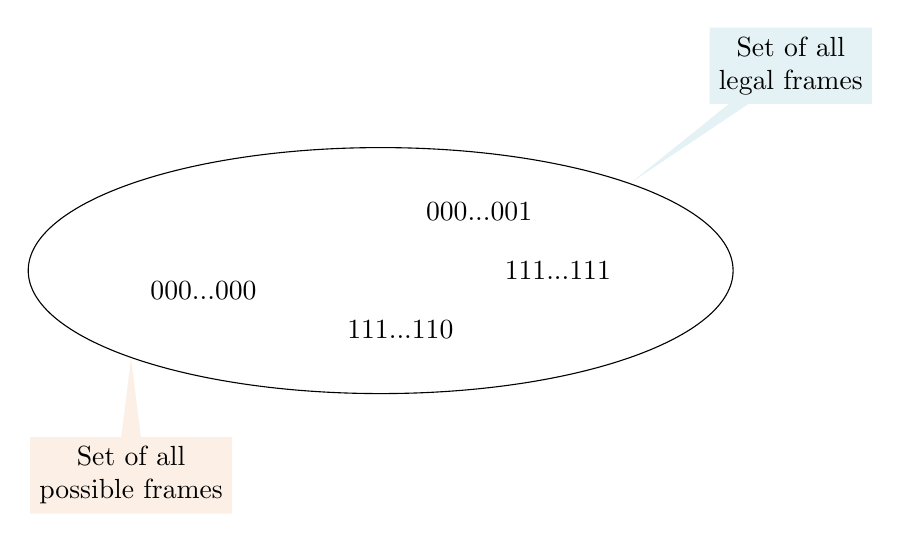
\begin{tikzpicture}
  \label{page:ll:allframes}

  \node (na) at (-0.5,0) {000...000}; 
  \node (nb) at (3,1) {000...001}; 
  \node (nc) at (2,-0.5) {111...110}; 
  \node (nd) at (4,0.25) {111...111}; 

  
  \node [draw, ellipse, fit=(na)(nb)(nc)(nd)] (allframes) {}; 

  \node [rectangle callout,
  fill=hpiblue!10, above right=of allframes, align=center,
  callout absolute pointer=(allframes.north east)] (alllegal) {Set of all \\ legal frames}; 

  \node [rectangle callout,
  fill=hpiorange!10, below=of allframes.south west, align=center,
  callout absolute pointer=(allframes.south west)] (alllegal) {Set of all \\ possible frames}; 

\end{tikzpicture}

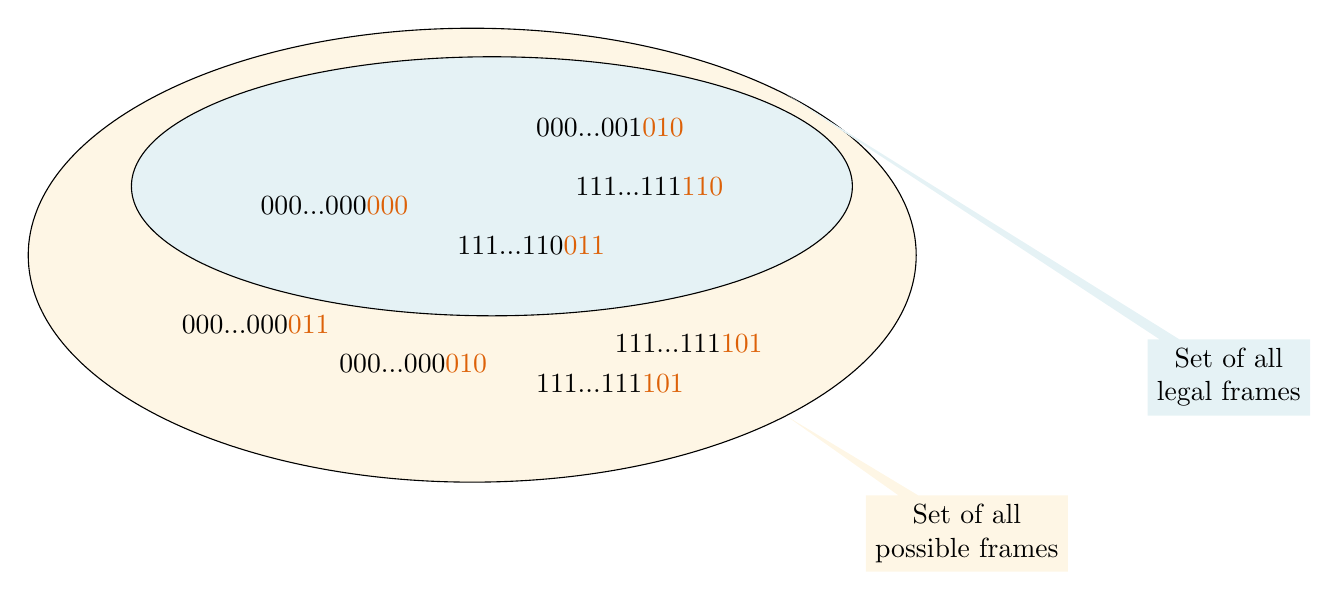
\begin{tikzpicture}
  \label{page:ll:legalframes}
  \node (na) at (-0.5,0) {000...000\color{hpiorange}{000}}; 
  \node (nb) at (3,1) {000...001\color{hpiorange}{010}}; 
  \node (nc) at (2,-0.5) {111...110\color{hpiorange}{011}}; 
  \node (nd) at (3.5,0.25) {111...111\color{hpiorange}{110}}; 

  \begin{scope}[on background layer]
  \end{scope}


  
  \node (nu) at (-1.5,-1.5) {000...000\color{hpiorange}{011}}; 
  \node (nv) at (0.5,-2) {000...000\color{hpiorange}{010}}; 
  \node (nw) at (3,-2.25) {111...111\color{hpiorange}{101}}; 
  \node (nx) at (4,-1.75) {111...111\color{hpiorange}{101}}; 


  \begin{scope}[on background layer]
    \node [draw, ellipse,  fill=hpiyellow!10, fit=(na)(nb)(nc)(nd)(nx)(nu)(nv)(nw), inner sep=5pt] (allframes) {}; 
    \node [draw, ellipse,  fill=hpiblue!10, fit=(na)(nb)(nc)(nd), inner sep=5pt] (alllegal) {}; 
  \end{scope}
  \node [rectangle callout,
  fill=hpiyellow!10, below right=of allframes, align=center,
  callout absolute pointer=(allframes.south east)] (alllegal) {Set of all \\ possible  frames}; 

  \node [rectangle callout,
  fill=hpiblue!10, above right=of alllegal, align=center,
  callout absolute pointer=(allframes.north east)] (alllegal) {Set of all \\ legal frames}; 

  
\end{tikzpicture}


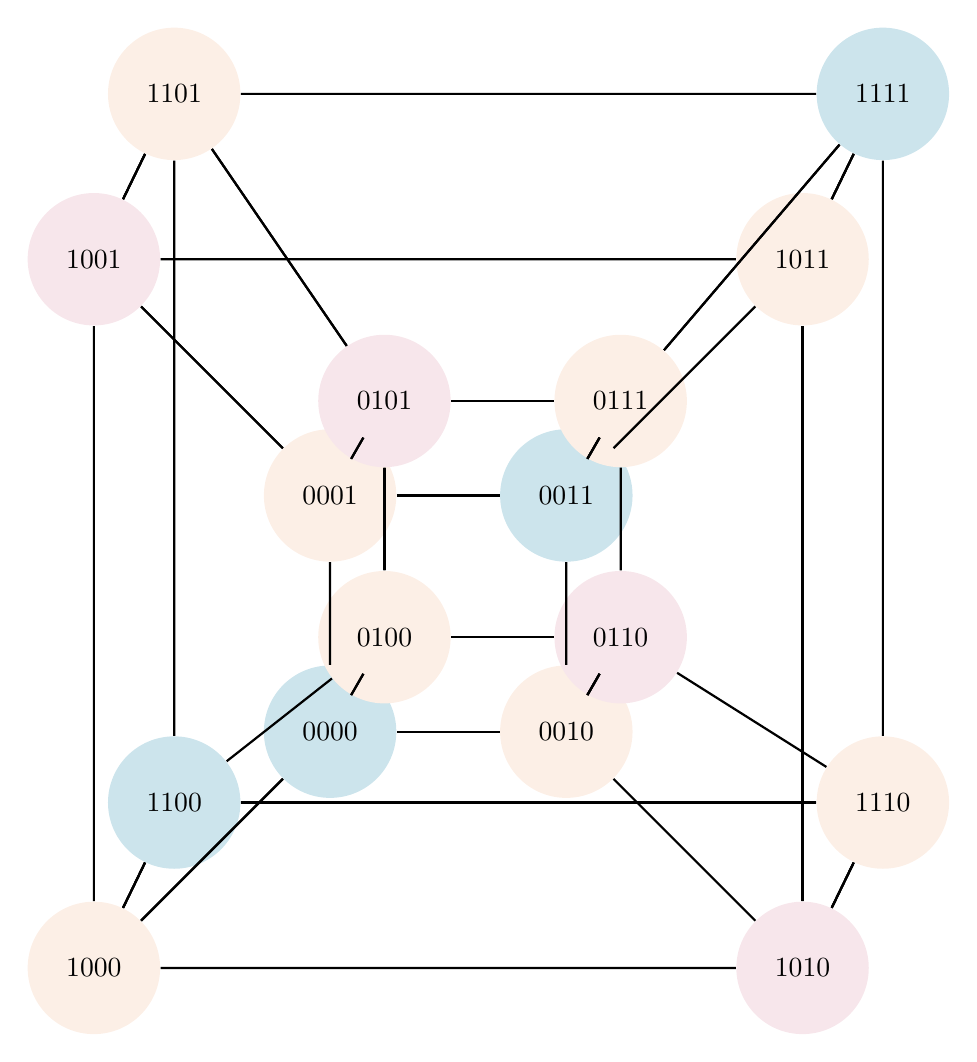
\begin{tikzpicture}[scale=3]
% based on https://texample.net/tikz/examples/gray-code-in-4-cube/
  
  \label{page:ll:altering_frames}

	 \tikzstyle{vertex}=[circle,minimum size=20pt,inner sep=0pt]
	 \tikzstyle{bad1vertex}=[circle,fill=hpiorange!10,inner sep=10pt]
	 \tikzstyle{bad2vertex}=[circle,fill=hpired!10,inner sep=10pt]
	 \tikzstyle{goodvertex}=[fill=hpiblue!20, circle, inner sep=10pt]
	 \tikzstyle{selected vertex} = [vertex, fill=red!24]
	 \tikzstyle{selected edge} = [draw,line width=5pt,-,red!50]
	 \tikzstyle{thin edge} = [draw,line width=2pt,-,red!50]
	 \tikzstyle{edge} = [draw,thick,-,black]
	 \node[goodvertex] (v0) at (0,0) {$0000$};
	 \node[bad1vertex] (v1) at (0,1) {$0001$};
	 \node[bad1vertex] (v2) at (1,0) {$0010$};
	 \node[goodvertex] (v3) at (1,1) {$0011$};
	 \node[bad1vertex] (v4) at (0.23, 0.4) {$0100$};
	 \node[bad2vertex] (v5) at (0.23,1.4) {$0101$};
	 \node[bad2vertex] (v6) at (1.23,0.4) {$0110$};
	 \node[bad1vertex] (v7) at (1.23,1.4) {$0111$};
	 \node[bad1vertex] (v8) at (-1,-1) {$1000$};
	 \node[bad2vertex] (v9) at (-1,2) {$1001$};
	 \node[bad1vertex] (v13) at (-0.66,2.7) {$1101$};
	 \node[goodvertex] (v12) at (-0.66,-0.3) {$1100$};
	 \node[bad2vertex] (v10) at (2,-1) {$1010$};
	 \node[bad1vertex] (v14) at (2.34,-0.3) {$1110$};
	 \node[bad1vertex] (v11) at (2,2) {$1011$};
	 \node[goodvertex] (v15) at (2.34,2.7) {$1111$};
	 \draw[edge] (v0) -- (v1) -- (v3) -- (v2) -- (v0);
	 \draw[edge] (v0) -- (v4) -- (v5) -- (v1) -- (v0);
	 \draw[edge] (v2) -- (v6) -- (v7) -- (v3) -- (v2);
	 \draw[edge] (v4) -- (v6) -- (v7) -- (v5) -- (v4);
	 \draw[edge] (v8) -- (v9) -- (v13) -- (v12) -- (v8);
	 \draw[edge] (v0) -- (v4) -- (v12) -- (v8) -- (v0);
	 \draw[edge] (v1) -- (v9) -- (v13) -- (v5) -- (v1);
	 \draw[edge] (v2) -- (v10) -- (v14) -- (v6) -- (v2);
	 \draw[edge] (v8) -- (v10) -- (v14) -- (v12) -- (v8);
	 \draw[edge] (v3) -- (v11) -- (v15) -- (v7) -- (v3);
	 \draw[edge] (v10) -- (v11) -- (v15) -- (v14) -- (v10);
	 \draw[edge] (v9) -- (v11) -- (v15) -- (v13) -- (v9);
	 \draw[edge] (v0) -- (v2);
	 \draw[edge] (v2) -- (v6);
	 \draw[edge] (v6) -- (v4);
	 \draw[edge] (v4) -- (v5);
	 \draw[edge] (v5) -- (v13);
	 \draw[edge] (v13) -- (v12);
	 \draw[edge] (v12) -- (v14);
	 \draw[edge] (v14) -- (v15);
	 \draw[edge] (v15) -- (v7);
	 \draw[edge] (v7) -- (v3);
	 \draw[edge] (v3) -- (v1);
	 \draw[edge] (v1) -- (v9);
	 \draw[edge] (v9) -- (v11);
	 \draw[edge] (v11) -- (v10);
	 \draw[edge] (v10) -- (v8);
	 \draw[edge] (v8) -- (v0);  
  
\end{tikzpicture}

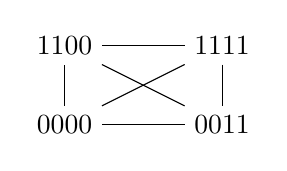
\begin{tikzpicture}
  \label{page:ll:simple_hamming:1}
  \node (a) at (0,0) {0000};
  \node (b) at (2,0) {0011};
  \node (c) at (0,1) {1100};
  \node (d) at (2,1) {1111};

  \draw (a) edge (b) edge (d) -- (c) edge (b) -- (d) --(b); 
\end{tikzpicture}


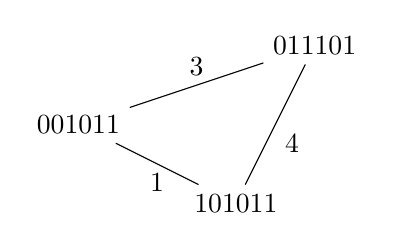
\begin{tikzpicture}
  \label{page:ll:simple_hamming:2}

  \node (a) at (0,0) {001011};
  \node (b) at (3,1) {011101};
  \node (c) at (2,-1) {101011};

  \draw (a) to node[above] {3} (b) to node[below right] {4} (c) to node [below] {1} (a); 
  
\end{tikzpicture}


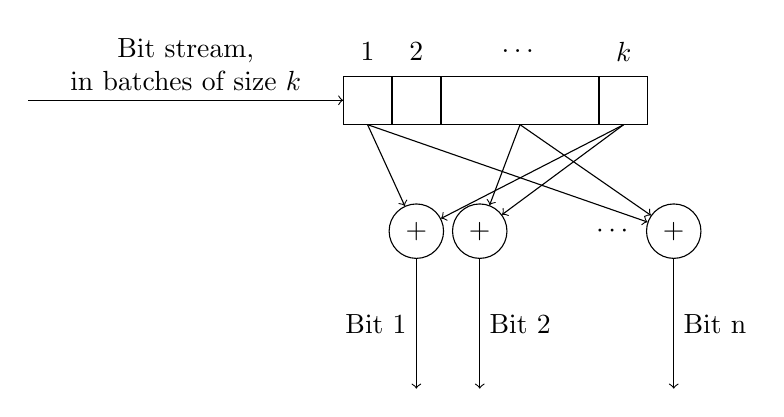
\begin{tikzpicture}
  \label{page:ll:block_code}
    \begin{scope}[every node/.style={draw, minimum width=4ex, minimum height=4ex}, node distance=0]
      \node [label=above:1] (n1) {}; 
      \node [label=above:2, right=of n1] (n2) {}; 
      \node [label=above:\dots, right=of n2, minimum width=2cm] (ndots) {}; 
      \node [label=above:$k$, right=of ndots] (nend) {}; 
    \end{scope}

   \draw [<-] (n1.west) to node[above,align=center]  {Bit stream,\\in batches of size $k$} ++(-4,0);

    \node [circle, draw, below= of n2] (p1) {+}; 
    \node [circle, draw, right=0.1 of p1] (p2) {+};
    \node [right=of p2] (pdots) {$\cdots$};
    \node [circle, draw, right=0.1 of pdots] (pend) {+};
    
    \draw [<-] (p1) edge (n1.south) edge (nend.south);
    \draw [<-] (p2) edge (ndots.south) edge (nend.south);
    \draw [<-] (pend) edge (n1.south) edge (ndots.south);

    \draw [->] (p1) to node[left] {Bit 1} ++(0, -2); 
    \draw [->] (p2) to node[right] {Bit 2} ++(0, -2); 
    \draw [->] (pend) to node[right] {Bit n} ++(0, -2); 
\end{tikzpicture}


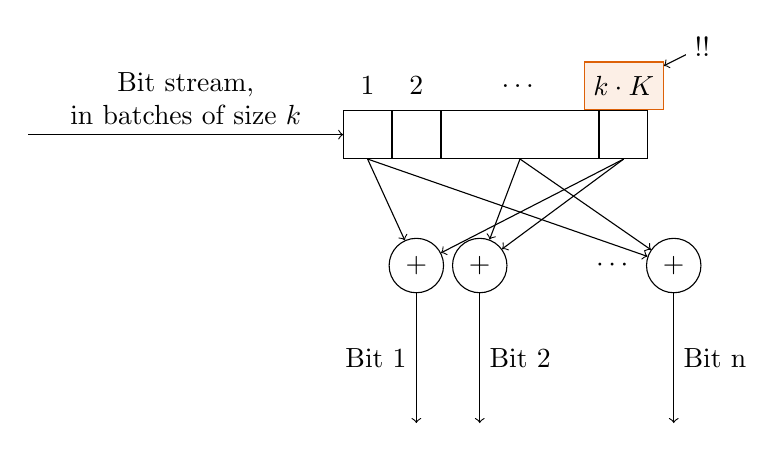
\begin{tikzpicture}
  \label{page:ll:convolutional_code}
    \begin{scope}[every node/.style={draw, minimum width=4ex, minimum height=4ex}, node distance=0]
      \node [label=above:1] (n1) {}; 
      \node [label=above:2, right=of n1] (n2) {}; 
      \node [label=above:\dots, right=of n2, minimum width=2cm] (ndots) {}; 
      \node [label={[above,fill=hpiorange!10,draw=hpiorange,name=kKlabel]:$k\cdot K$}, right=of ndots] (nend) {}; 
    \end{scope}

    \draw [<-] (kKlabel) -- ++(1,0.5) node[fill=white] {!!}; 
    
    
   \draw [<-] (n1.west) to node[above,align=center]  {Bit stream,\\in batches of size $k$} ++(-4,0);

    \node [circle, draw, below= of n2] (p1) {+}; 
    \node [circle, draw, right=0.1 of p1] (p2) {+};
    \node [right=of p2] (pdots) {$\cdots$};
    \node [circle, draw, right=0.1 of pdots] (pend) {+};
    
    \draw [<-] (p1) edge (n1.south) edge (nend.south);
    \draw [<-] (p2) edge (ndots.south) edge (nend.south);
    \draw [<-] (pend) edge (n1.south) edge (ndots.south);

    \draw [->] (p1) to node[left] {Bit 1} ++(0, -2); 
    \draw [->] (p2) to node[right] {Bit 2} ++(0, -2); 
    \draw [->] (pend) to node[right] {Bit n} ++(0, -2); 
\end{tikzpicture}


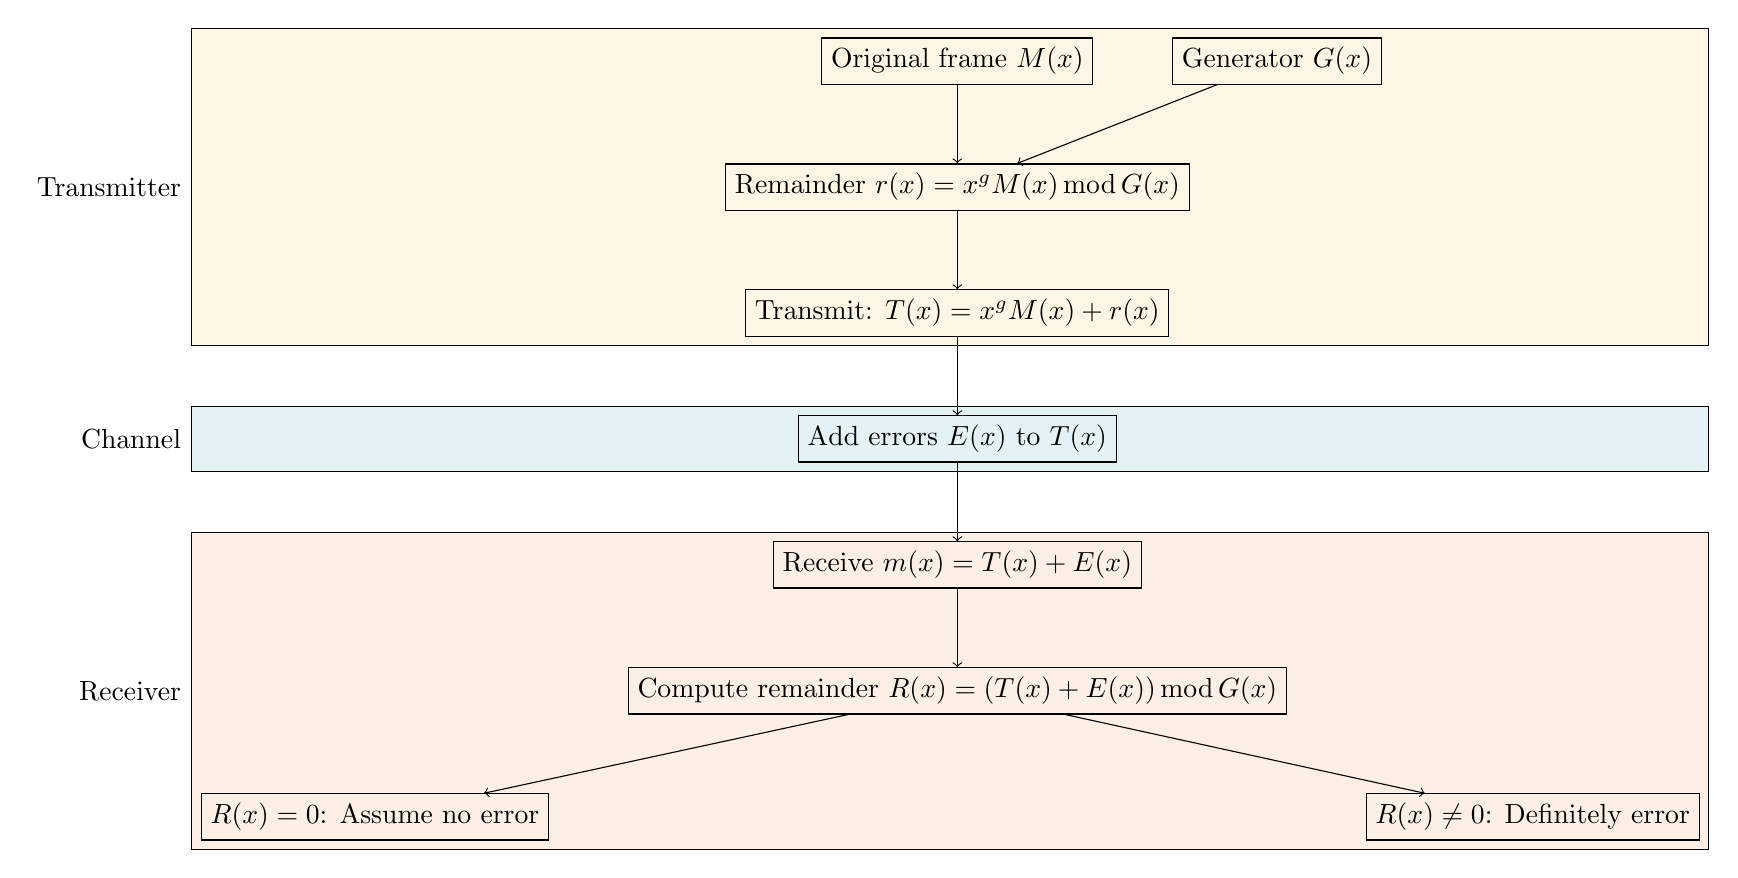
\begin{tikzpicture}[every node/.style={draw}]
  \label{page:ll:crc}
  
  \node (frame) {Original frame $M(x)$ };
  \node [right=of frame] (generator) {Generator $G(x)$};
  \node [below=of frame] (remainder) {Remainder $r(x) = x^g M(x) \, \mathrm{mod}\, G(x)$};

  \node [below =of remainder] (transmit) {Transmit: $T(x) = x^g M(x) + r(x)$};
  
  \node [below=of transmit] (channel) {Add errors $E(x)$ to $T(x)$};

  \node [below=of channel] (receive) {Receive $m(x) = T(x) + E(x)$};
  \node [below=of receive] (compute) {Compute remainder $ R(x)  = (T(x) + E(x)) \,\mathrm{mod} \, G(x)$};

  \node [below left=of compute] (noerror) {$R(x) = 0$: Assume no error};
  \node [below right=of compute] (error) {$R(x) \not = 0$: Definitely error};

  \draw [->] (frame) edge (remainder) (generator) edge (remainder) (remainder) edge (transmit) (transmit) edge (channel) (channel) edge (receive) (receive) edge (compute) (compute) edge (noerror)  (compute) edge (error); 

  \begin{scope}[on background layer]
    \node [fill=hpiyellow!10, fit=(frame)(generator)(transmit)(transmit.south -| noerror.west)(transmit.south -| error.east), label=left:Transmitter ] { }; 
    \node [fill=hpiblue!10, fit=(channel)(channel.south -| noerror.west)(channel.south -| error.east), label=left:Channel ] { }; 
    \node [fill=hpiorange!10, fit=(receive)(noerror)(error), label=left:Receiver ] { }; 
    
  \end{scope}
  
\end{tikzpicture}

\end{document}